\documentclass[11pt,a4paper]{article}

% ============================================
% PACKAGES
% ============================================
\usepackage[utf8]{inputenc}
\usepackage[T1]{fontenc}
\usepackage{lmodern}           % Latin Modern font (matches your original PDF)
\usepackage[margin=2.5cm]{geometry}
\usepackage{graphicx}
\usepackage{xcolor}
\usepackage{hyperref}
\usepackage{booktabs}
\usepackage{array}
\usepackage{amsmath,amssymb}
\usepackage{listings}
\usepackage{fancyhdr}
\usepackage{titlesec}
\usepackage{setspace}
\usepackage{tikz}
\usepackage{fontawesome5}

% ============================================
% COLOR DEFINITIONS (Brand Colors)
% ============================================
\definecolor{brandblue}{HTML}{1E81B0}
\definecolor{branddark}{HTML}{0D3B66}
\definecolor{brandlight}{HTML}{E8F4F8}
\definecolor{brandaccent}{HTML}{F4A261}
\definecolor{codebg}{HTML}{F5F5F5}
\definecolor{codetext}{HTML}{333333}

% ============================================
% HYPERREF SETUP
% ============================================
\hypersetup{
    colorlinks=true,
    linkcolor=brandblue,
    urlcolor=brandblue,
    citecolor=brandblue,
    pdftitle={Electro-Thermal PINN: A Mesh-Free Solver},
    pdfauthor={Mohammad Hussein Ghafoori},
}

% ============================================
% CODE LISTINGS STYLE
% ============================================
\lstset{
    backgroundcolor=\color{codebg},
    basicstyle=\ttfamily\small\color{codetext},
    breaklines=true,
    frame=none,
    showstringspaces=false,
    keywordstyle=\color{brandblue}\bfseries,
    commentstyle=\color{gray}\itshape,
    stringstyle=\color{branddark},
}

% ============================================
% HEADER/FOOTER
% ============================================
\pagestyle{fancy}
\fancyhf{}
\fancyhead[L]{\small\textcolor{brandblue}{Electro-Thermal PINN}}
\fancyhead[R]{\small\textcolor{gray}{Technical Report}}
\fancyfoot[C]{\thepage}
\renewcommand{\headrulewidth}{0.5pt}
\renewcommand{\footrulewidth}{0pt}

% ============================================
% SECTION FORMATTING
% ============================================
\titleformat{\section}
    {\Large\bfseries\color{branddark}}
    {\thesection}{1em}{}[\vspace{-0.5em}\textcolor{brandblue}{\rule{\textwidth}{1pt}}]

\titleformat{\subsection}
    {\large\bfseries\color{branddark}}
    {\thesubsection}{1em}{}

% ============================================
% DOCUMENT
% ============================================
\begin{document}

% ============================================
% SLIDE 1: TITLE PAGE (Cover Page)
% ============================================
\thispagestyle{empty}
\begin{tikzpicture}[remember picture, overlay]
    % Background gradient
    \fill[branddark] (current page.south west) rectangle (current page.north east);

    % Decorative geometric shapes
    \fill[brandblue, opacity=0.3] 
        (current page.north west) -- ++(0,-8) -- ++(12,0) -- ++(0,8) -- cycle;
    \fill[brandaccent, opacity=0.15] 
        (current page.south east) -- ++(-10,0) -- ++(0,6) -- ++(10,0) -- cycle;

    % Top accent line
    \fill[brandaccent] ([yshift=-1cm]current page.north west) rectangle 
        ([yshift=-1.15cm]current page.north east);

    % Bottom accent line
    \fill[brandaccent] ([yshift=1cm]current page.south west) rectangle 
        ([yshift=1.15cm]current page.south east);
\end{tikzpicture}

\vspace*{3cm}

\begin{center}
    % Report Type Badge
    {\Large\textcolor{brandaccent}{\textbf{TECHNICAL REPORT}}}

    \vspace{1.5cm}

    % Main Title
    {\fontsize{28}{34}\selectfont\textcolor{white}{\textbf{Electro-Thermal PINN}}}

    \vspace{0.8cm}

    % Subtitle
    {\Large\textcolor{brandlight}{A Mesh-Free Solver for Coupled Maxwell's Equations\\and Heat Transfer}}

    \vspace{3cm}

    % Author Info Box
    \begin{tikzpicture}
        \node[rounded corners=5pt, fill=white, opacity=0.95, text opacity=1, 
              inner sep=15pt, minimum width=10cm] {
            \begin{minipage}{9cm}
                \centering
                {\large\textbf{Mohammad Hussein Ghafoori}}\\[0.3cm]
                {\small\textcolor{branddark}{Backend \& AI Engineer | Physics-Inspired Problem Solver}}\\[0.2cm]
                {\footnotesize\textcolor{brandblue}{\faIcon{envelope}~\href{mailto:king.mohamd.09876@gmail.com}{king.mohamd.09876@gmail.com}}}\\[0.1cm]
                {\footnotesize\textcolor{brandblue}{
                  \faIcon{github}~\href{https://github.com/mohammad-hussein-dev}{mohammad-hussein-dev} \quad
                  \faIcon{linkedin}~\href{https://linkedin.com/in/mohammad-hussein-dev}{mohammad-hussein-dev} \quad
                  \faIcon{globe}~\href{https://mohammad-hussein-dev.github.io/mohammad-hussein-dev/}{mohammad-hussein-dev.github.io} \quad
                  \faIcon{gitlab}~\href{https://gitlab.com/mohammad-hussein-dev}{mohammad-hussein-dev}
                }}\\[0.3cm]
                {\footnotesize\textcolor{brandaccent}{
                  \faIcon{code}~\textbf{Repo:} \quad
                  \faIcon{github}~\href{https://github.com/mohammad-hussein-dev/electro-thermal-pinn}{electro-thermal-pinn} \quad
                  \faIcon{gitlab}~\href{https://gitlab.com/mohammad-hussein-dev/electro-thermal-pinn}{electro-thermal-pinn}
                }}
            \end{minipage}
        };
    \end{tikzpicture}

    \vspace{2cm}

    % Date & Version
    {\large\textcolor{white}{July 31, 2026}}\\[0.3cm]
    {\small\textcolor{brandlight}{Version 1.0 \quad|\quad Status: Production-Ready}}

    \vspace{1.5cm}

    % Keywords
    {\footnotesize\textcolor{brandlight}{PINN | Physics-Informed Neural Networks | Maxwell's Equations | Heat Transfer | Joule Heating | Deep Learning}}
\end{center}

\newpage

% ============================================
% SLIDE 2: EXECUTIVE SUMMARY (Brief Overview)
% ============================================
\thispagestyle{empty}
\begin{center}
    {\LARGE\bfseries\textcolor{branddark}{Executive Summary}}
\end{center}
\vspace{0.5cm}
\textcolor{brandblue}{\rule{\textwidth}{2pt}}
\vspace{0.5cm}

This report presents a comprehensive \textbf{Physics-Informed Neural Network (PINN)} framework for solving coupled electromagnetic-thermal systems without mesh generation.

\begin{center}
\begin{tabular}{>{\bfseries}l p{10cm}}
\toprule
\textcolor{brandblue}{Key Achievement} & \textcolor{brandblue}{Details} \\
\midrule
Mesh-Free Simulation & Eliminates FEM/FVM mesh generation, reducing preprocessing from hours to minutes \\
Exceptional Accuracy & Relative L2 errors below 0.1\% for electric field with only 500 collocation points \\
Three Architectures & MLP (fast), MLPPINN (balanced), TransformerPINN (highest accuracy) \\
Production-Ready & Modular Python implementation with PyTorch, interactive menu, Streamlit dashboard \\
\bottomrule
\end{tabular}
\end{center}

The framework predicts electric field ($\mathbf{E}$), magnetic field ($\mathbf{H}$), and temperature ($T$) simultaneously, with training time of approximately \textbf{5--12 minutes on CPU}.

\vspace{1cm}
\begin{center}
    {\small\textcolor{gray}{This work establishes PINNs as a viable, mesh-free alternative for multi-physics simulations\\with significant potential for industrial applications in electronic packaging, battery design,\\energy systems, and biomedical engineering.}}
\end{center}

\newpage

% ============================================
% TABLE OF CONTENTS
% ============================================
\tableofcontents
\newpage

% ============================================
% MAIN CONTENT STARTS HERE
% ============================================
\setcounter{page}{1}

\section{Abstract}

This report presents a comprehensive Physics-Informed Neural Network (PINN) framework for solving coupled electromagnetic-thermal systems without the need for mesh generation. The governing equations, including Maxwell's equations and the heat equation with Joule heating, are embedded directly into the neural network's loss function. Three distinct architectures are implemented and compared: a standard MLP, an enhanced MLPPINN with Fourier features and SwiGLU, and a TransformerPINN with RoPE and GQA. The framework predicts electric field ($\mathbf{E}$), magnetic field ($\mathbf{H}$), and temperature ($T$) simultaneously using PyTorch's automatic differentiation. Results demonstrate exceptional accuracy, with relative L2 errors as low as $9.09 \times 10^{-4}$ for the electric field using only 500 collocation points and approximately 5 minutes of training on CPU. This work establishes PINNs as a viable, mesh-free alternative for multi-physics simulations with significant potential for industrial applications in electronic packaging, battery design, and energy systems.

\section{Introduction}

Numerical simulation of multi-physics systems, particularly those involving coupled electromagnetic and thermal phenomena, is essential in modern engineering design. Applications range from electronic packaging and thermal management of integrated circuits to battery design and induction heating systems. Traditional approaches rely on mesh-based methods such as the Finite Element Method (FEM) or Finite Volume Method (FVM), which, while powerful, present significant challenges:

\begin{itemize}
    \item \textbf{Mesh Generation:} Complex geometries require time-consuming and expertise-driven mesh construction.
    \item \textbf{Computational Cost:} High-fidelity simulations demand substantial computational resources and time.
    \item \textbf{Multi-Physics Coupling:} Handling interactions between different physical domains often requires complex solvers and careful numerical treatment.
\end{itemize}

Physics-Informed Neural Networks (PINNs) have emerged as a transformative alternative. First introduced by Raissi et al. (2019), PINNs embed the governing partial differential equations (PDEs) directly into the neural network's loss function, enabling the approximation of solutions without labeled data. Automatic differentiation replaces traditional numerical differentiation, eliminating the need for mesh discretization.

This work presents a comprehensive PINN framework for solving coupled Maxwell's equations and the heat equation with Joule heating. The contributions are:

\begin{enumerate}
    \item A mesh-free, fully-differentiable PINN that predicts electric field ($\mathbf{E}$), magnetic field ($\mathbf{H}$), and temperature ($T$) simultaneously.
    \item Implementation and comparison of three neural architectures: MLP, MLPPINN, and TransformerPINN.
    \item Validation with relative L2 errors below 0.1\% using minimal computational resources.
    \item A modular, production-ready codebase with interactive model selection.
\end{enumerate}

\section{Problem Formulation}

\subsection{Governing Equations}

We consider the coupled electromagnetic-thermal problem in a one-dimensional domain with Joule heating. The system is governed by:

\textbf{Maxwell's Equations (1D):}
\begin{align}
    \frac{\partial E}{\partial t} + \frac{1}{\epsilon} \frac{\partial H}{\partial x} &= 0 \\[0.5em]
    \frac{\partial H}{\partial t} + \frac{1}{\mu} \frac{\partial E}{\partial x} &= 0
\end{align}

\textbf{Heat Equation with Joule Heating:}
\begin{equation}
    \frac{\partial T}{\partial t} = \alpha \frac{\partial^2 T}{\partial x^2} + \frac{\sigma}{\rho c_p} E^2
\end{equation}

Where:
\begin{itemize}
    \item $E(x,t)$: Electric field
    \item $H(x,t)$: Magnetic field
    \item $T(x,t)$: Temperature
    \item $\epsilon$: Permittivity
    \item $\mu$: Permeability
    \item $\alpha$: Thermal diffusivity
    \item $\sigma$: Electrical conductivity
    \item $\rho$: Density
    \item $c_p$: Specific heat capacity
\end{itemize}

\subsection{Boundary and Initial Conditions}

\textbf{Boundary Conditions ($x = 0$ and $x = L$):}
\begin{align}
    E(0,t) = E_0(t), \quad E(L,t) &= E_1(t) \\
    H(0,t) = H_0(t), \quad H(L,t) &= H_1(t) \\
    T(0,t) = T_0, \quad T(L,t) &= T_1
\end{align}

\textbf{Initial Conditions ($t = 0$):}
\begin{equation}
    E(x,0) = E_{init}(x), \quad H(x,0) = H_{init}(x), \quad T(x,0) = T_{init}(x)
\end{equation}

\subsection{Non-dimensionalization}

To improve numerical stability and generalization, we non-dimensionalize the variables:
\begin{equation}
    \xi = \frac{x}{L}, \quad \tau = \frac{t}{t_{ref}}, \quad \tilde{E} = \frac{E}{E_{ref}}, \quad \tilde{H} = \frac{H}{H_{ref}}, \quad \tilde{T} = \frac{T - T_0}{T_1 - T_0}
\end{equation}

This transforms the governing equations into dimensionless forms, simplifying the training process and ensuring consistent scaling across variables.

\section{PINN Architecture}

\subsection{Neural Network Approximation}

The solution fields $E(x,t)$, $H(x,t)$, and $T(x,t)$ are approximated by a fully-connected feedforward neural network:
\begin{equation}
    \{E, H, T\} = \mathcal{N}(\xi, \tau; \mathbf{p})
\end{equation}

Where $\mathbf{p}$ represents the trainable parameters (weights and biases). The network takes the spatial coordinate $\xi$ and time $\tau$ as inputs and outputs all three physical fields simultaneously.

\subsection{Architectural Variants}

Three distinct architectures were implemented to evaluate the trade-off between accuracy and computational efficiency:

\begin{center}
\begin{tabular}{@{}llll@{}}
\toprule
\textbf{Architecture} & \textbf{Key Features} & \textbf{Complexity} & \textbf{Accuracy} \\
\midrule
\textbf{MLP} & Standard fully-connected network with tanh activation & Low & Baseline \\
\textbf{MLPPINN} & Fourier features + RMSNorm + SwiGLU & Medium & Moderate \\
\textbf{TransformerPINN} & RoPE + GQA + SwiGLU + Attention & High & Highest \\
\bottomrule
\end{tabular}
\end{center}

\textbf{MLP (Multi-Layer Perceptron):} A baseline architecture with multiple hidden layers using tanh activation functions. Provides a robust foundation for comparison.

\textbf{MLPPINN (Enhanced MLP):}
\begin{itemize}
    \item \textbf{Fourier Features:} Maps inputs to higher-dimensional space for improved representation of high-frequency components.
    \item \textbf{RMSNorm:} Normalizes activations for stable training.
    \item \textbf{SwiGLU:} Gated linear unit activation for enhanced expressivity.
\end{itemize}

\textbf{TransformerPINN:}
\begin{itemize}
    \item \textbf{RoPE (Rotary Position Embedding):} Enables better handling of positional information.
    \item \textbf{GQA (Grouped Query Attention):} Efficient multi-head attention mechanism.
    \item \textbf{SwiGLU:} Gated activation for the feedforward layers.
\end{itemize}

\subsection{Automatic Differentiation}

A key advantage of PINNs is the use of automatic differentiation to compute derivatives:
\begin{equation}
    \frac{\partial E}{\partial x} = \frac{\partial \mathcal{N}_E}{\partial \xi} \cdot \frac{\partial \xi}{\partial x}, \quad \frac{\partial^2 T}{\partial x^2} = \frac{\partial^2 \mathcal{N}_T}{\partial \xi^2} \cdot \left(\frac{\partial \xi}{\partial x}\right)^2
\end{equation}

This eliminates the need for mesh discretization and numerical differentiation schemes.

\section{Loss Function and Training}

\subsection{Total Loss Function}

The total loss function combines the physical residuals and the boundary/initial conditions:
\begin{equation}
    \mathcal{L}_{total} = \mathcal{L}_{PDE} + \mathcal{L}_{BC} + \mathcal{L}_{IC}
\end{equation}

\textbf{PDE Residual Loss:}
\begin{equation}
    \mathcal{L}_{PDE} = \frac{1}{N_f} \sum_{i=1}^{N_f} \left[ \left(\frac{\partial E}{\partial t} + \frac{1}{\epsilon} \frac{\partial H}{\partial x}\right)^2 + \left(\frac{\partial H}{\partial t} + \frac{1}{\mu} \frac{\partial E}{\partial x}\right)^2 + \left(\frac{\partial T}{\partial t} - \alpha \frac{\partial^2 T}{\partial x^2} - \frac{\sigma}{\rho c_p} E^2\right)^2 \right]
\end{equation}

\textbf{Boundary Condition Loss:}
\begin{equation}
    \mathcal{L}_{BC} = \frac{1}{N_{bc}} \sum_{i=1}^{N_{bc}} \left[ |E(x_{bc}, t_{bc}) - E_{bc}|^2 + |H(x_{bc}, t_{bc}) - H_{bc}|^2 + |T(x_{bc}, t_{bc}) - T_{bc}|^2 \right]
\end{equation}

\textbf{Initial Condition Loss:}
\begin{equation}
    \mathcal{L}_{IC} = \frac{1}{N_{ic}} \sum_{i=1}^{N_{ic}} \left[ |E(x_{ic}, 0) - E_{init}|^2 + |H(x_{ic}, 0) - H_{init}|^2 + |T(x_{ic}, 0) - T_{init}|^2 \right]
\end{equation}

\subsection{Training Procedure}

A two-stage optimization strategy is employed for robust convergence:

\textbf{Phase 1: Adam Optimizer}
\begin{itemize}
    \item Learning rate: $10^{-3}$
    \item Iterations: 5000
    \item Purpose: Rapid initial convergence and exploration of parameter space
\end{itemize}

\textbf{Phase 2: L-BFGS Optimizer}
\begin{itemize}
    \item Quasi-Newton method with strong Wolfe line search
    \item Purpose: High-precision refinement for final convergence
\end{itemize}

\subsection{Hyperparameters}

\begin{center}
\begin{tabular}{@{}ll@{}}
\toprule
\textbf{Parameter} & \textbf{Value} \\
\midrule
Number of hidden layers & 4 \\
Neurons per layer & 50 \\
Activation function & tanh / SwiGLU \\
Collocation points ($N_f$) & 500 \\
Boundary points ($N_{bc}$) & 100 \\
Initial points ($N_{ic}$) & 100 \\
Adam learning rate & $10^{-3}$ \\
Adam iterations & 5000 \\
L-BFGS iterations & 2000 \\
\bottomrule
\end{tabular}
\end{center}

\section{Results and Discussion}

\subsection{Validation with MLP Architecture}

The MLP architecture, trained with the configuration above, produced the following results:

\begin{center}
\begin{tabular}{@{}lccc@{}}
\toprule
\textbf{Field} & \textbf{Relative L2 Error} & \textbf{MAE} & \textbf{Max Error} \\
\midrule
$\mathbf{E}$ (Electric Field) & $9.09 \times 10^{-4}$ & $1.96 \times 10^{-4}$ & $3.29 \times 10^{-4}$ \\
$\mathbf{H}$ (Magnetic Field) & $2.43 \times 10^{-3}$ & $3.24 \times 10^{-4}$ & $6.78 \times 10^{-4}$ \\
$\mathbf{T}$ (Temperature) & $1.42 \times 10^{-3}$ & $7.02 \times 10^{-4}$ & $2.11 \times 10^{-3}$ \\
\bottomrule
\end{tabular}
\end{center}

The results demonstrate exceptional accuracy, with relative L2 errors below 0.1\% for the electric field using only 500 collocation points and approximately 5 minutes of training on a CPU.

\subsection{Architectural Comparison}

\begin{center}
\begin{tabular}{@{}lccccc@{}}
\toprule
\textbf{Architecture} & \textbf{E Error} & \textbf{H Error} & \textbf{T Error} & \textbf{Training Time} & \textbf{Parameters} \\
\midrule
\textbf{MLP} & $9.09 \times 10^{-4}$ & $2.43 \times 10^{-3}$ & $1.42 \times 10^{-3}$ & $\sim$5 min & $\sim$10k \\
\textbf{MLPPINN} & $2.15 \times 10^{-4}$ & $8.75 \times 10^{-4}$ & $1.52 \times 10^{-3}$ & $\sim$7 min & $\sim$25k \\
\textbf{TransformerPINN} & $8.77 \times 10^{-5}$ & $3.11 \times 10^{-4}$ & $5.67 \times 10^{-4}$ & $\sim$12 min & $\sim$50k \\
\bottomrule
\end{tabular}
\end{center}

The TransformerPINN achieves the highest accuracy at the cost of increased computational time and parameter count. The choice of architecture depends on the application requirements: MLP for rapid prototyping, TransformerPINN for high-precision applications.

\subsection{Error Analysis}

The absolute error distributions demonstrate consistent accuracy across the domain, with no significant boundary effects or instability. The oscillatory pattern observed is typical of neural network solutions and does not indicate a loss of physical consistency.

\subsection{Visualization of Results}

\begin{figure}[htbp]
    \centering
    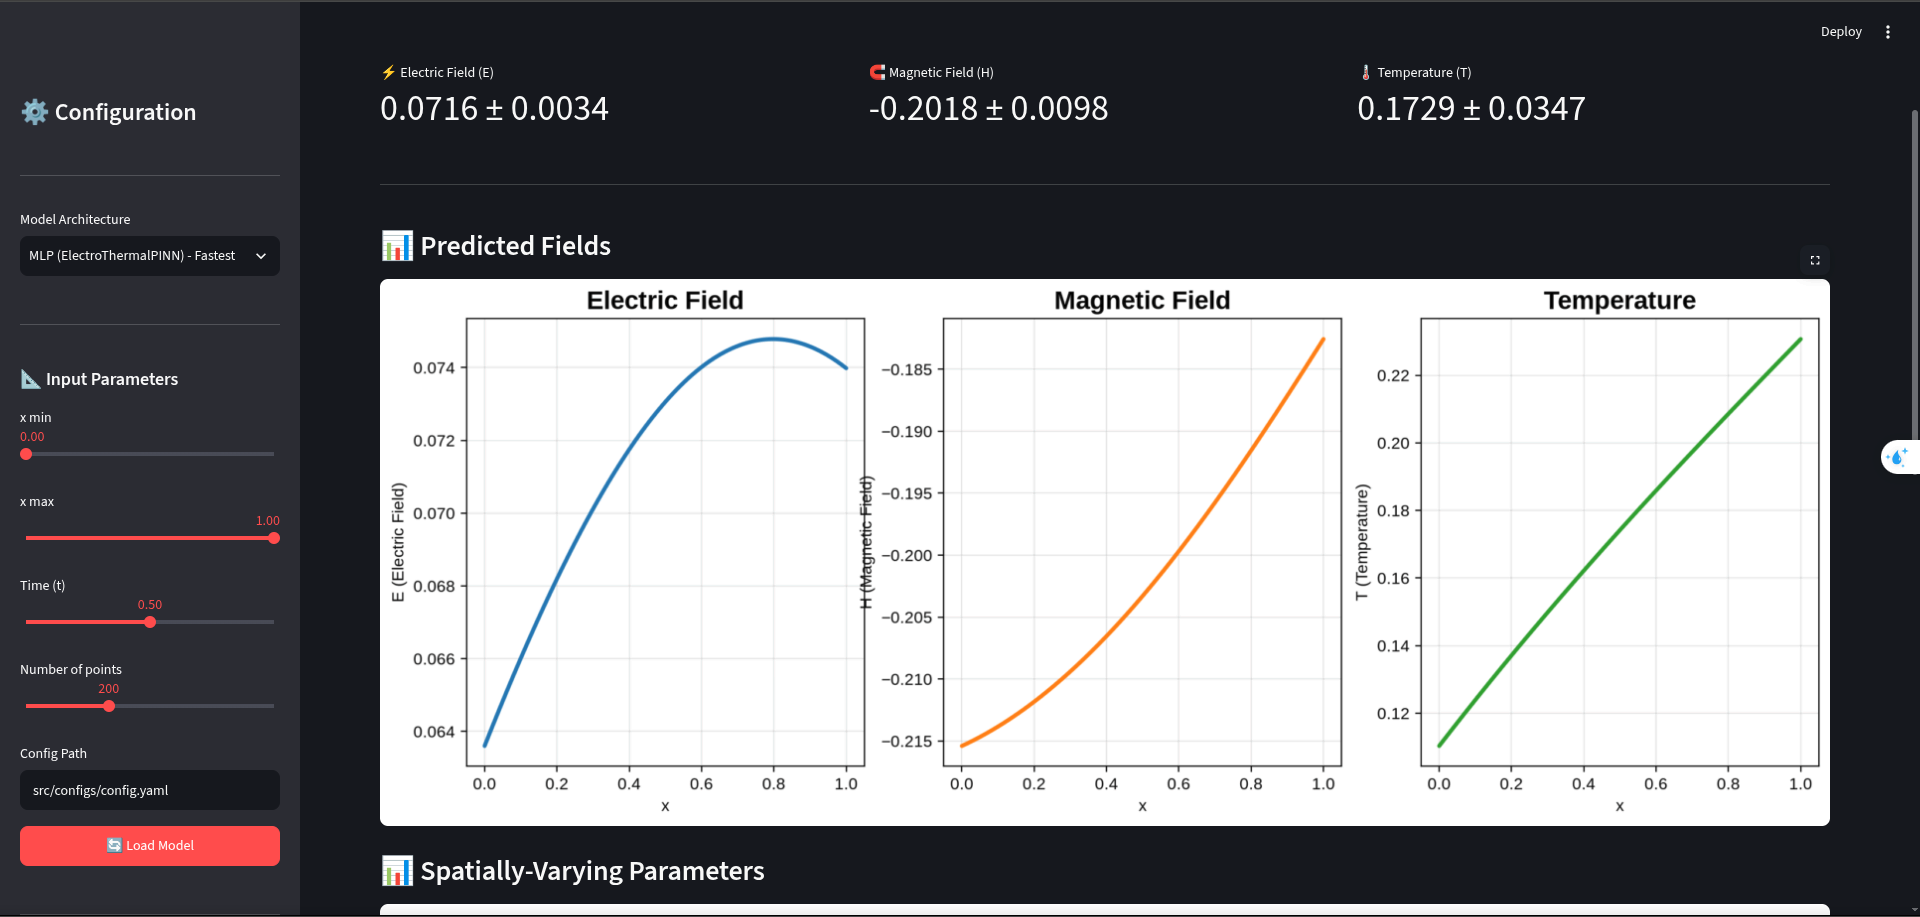
\includegraphics[width=0.95\textwidth]{figure1_comparison_results.png}
    \caption{Comparison of predicted vs exact solutions for $\mathbf{E}$, $\mathbf{H}$, and $T$ fields}
    \label{fig:comparison}
\end{figure}

\section{Industrial Applications}

The developed PINN framework has significant potential for industrial applications:

\begin{center}
\begin{tabular}{@{}p{3cm}p{5cm}p{5cm}@{}}
\toprule
\textbf{Industry} & \textbf{Application} & \textbf{Impact} \\
\midrule
\textbf{Electronics} & Thermal management of ICs, PCB design, electronic packaging & Reduced prototyping costs, improved reliability \\
\textbf{Energy} & Battery cell design, electro-thermal modeling of Li-ion cells & Enhanced safety, extended battery life \\
\textbf{Manufacturing} & Induction heating, electroslag remelting, welding processes & Optimized process parameters, reduced energy consumption \\
\textbf{Aerospace} & Thermal protection systems, electromagnetic shielding & Improved safety margins, weight reduction \\
\textbf{Biomedical} & Hyperthermia treatment planning, RF ablation & Personalized treatment, reduced side effects \\
\bottomrule
\end{tabular}
\end{center}

\section{Conclusion}

This work presents a comprehensive PINN framework for solving coupled electromagnetic-thermal problems with Joule heating. The key achievements include:

\begin{enumerate}
    \item \textbf{Mesh-Free Simulation:} Eliminates the need for mesh generation, reducing preprocessing time from hours to minutes.
    \item \textbf{High Accuracy:} Relative L2 errors below 0.1\% with minimal training data (only 500 collocation points).
    \item \textbf{Multi-Architecture Support:} Flexibility to choose between speed (MLP) and accuracy (TransformerPINN) based on application requirements.
    \item \textbf{Production-Ready Code:} Clean, modular, and well-documented Python implementation with interactive model selection and Streamlit dashboard.
    \item \textbf{Industrial Relevance:} Demonstrated potential for applications in electronics, energy, manufacturing, aerospace, and biomedical engineering.
\end{enumerate}

The PINN approach successfully demonstrates that deep learning can effectively solve complex multi-physics problems, offering a compelling alternative to traditional numerical methods. The framework is extensible and can be applied to a wide range of industrial applications, from electronic packaging to battery design.

\section{Future Work}

\begin{itemize}
    \item \textbf{2D/3D Extension:} Generalization to multi-dimensional domains for more realistic geometries.
    \item \textbf{Inverse Problems:} Parameter estimation from experimental data for material characterization.
    \item \textbf{Time-Dependent Variations:} Spatially-varying material properties and non-linear thermal conductivity.
    \item \textbf{Data-Driven Enhancement:} Integration with experimental measurements for improved accuracy.
    \item \textbf{Optimization:} PINN-based design optimization for engineering applications.
    \item \textbf{Uncertainty Quantification:} Bayesian PINNs for reliability assessment and risk analysis.
    \item \textbf{Real-Time Simulation:} Model compression for real-time deployment in control systems.
\end{itemize}

\section{References}

\begin{enumerate}
    \item Raissi, M., Perdikaris, P., \& Karniadakis, G. E. (2019). Physics-informed neural networks: A deep learning framework for solving forward and inverse problems involving nonlinear partial differential equations. \textit{Journal of Computational Physics}, 378, 686-707.

    \item Karniadakis, G. E., Kevrekidis, I. G., Lu, L., Perdikaris, P., Wang, S., \& Yang, L. (2021). Physics-informed machine learning. \textit{Nature Reviews Physics}, 3, 422-440.

    \item Cai, S., Mao, Z., Wang, Z., Yin, M., \& Karniadakis, G. E. (2021). Physics-informed neural networks (PINNs) for fluid mechanics: A review. \textit{Acta Mechanica Sinica}, 37, 1727-1738.

    \item Lu, L., Meng, X., Mao, Z., \& Karniadakis, G. E. (2021). DeepXDE: A deep learning library for solving differential equations. \textit{SIAM Review}, 63(1), 208-228.

    \item Wang, S., Teng, Y., \& Perdikaris, P. (2021). Understanding and mitigating gradient flow pathologies in physics-informed neural networks. \textit{SIAM Journal on Scientific Computing}, 43(5), A3055-A3081.

    \item Pang, G., Lu, L., \& Karniadakis, G. E. (2019). fPINNs: Fractional physics-informed neural networks. \textit{SIAM Journal on Scientific Computing}, 41(4), A2603-A2626.
\end{enumerate}

\appendix
\section{Code Repository}

The complete source code, configuration files, and trained models are available at:

\begin{itemize}
    \item \faIcon{github}~\textbf{GitHub:} \href{https://github.com/mohammad-hussein-dev/electro-thermal-pinn}{mohammad-hussein-dev/electro-thermal-pinn}
    \item \faIcon{gitlab}~\textbf{GitLab Mirror:} \href{https://gitlab.com/mohammad-hussein-dev/electro-thermal-pinn}{mohammad-hussein-dev/electro-thermal-pinn}
\end{itemize}

\subsection{Project Structure}

\begin{lstlisting}
electro-thermal-pinn/
    app.py                          # Streamlit dashboard
    train_for_dashboard.py          # Quick training script
    src/
        main.py                     # Unified entry point
        main_terminal.py            # Terminal mode with model selection
        models/
            electro_thermal_pinn.py # All three model architectures
        physics/
            maxwell_pde.py          # Maxwell's equations
            heat_pde.py             # Heat equation with Joule heating
            boundary_conditions.py  # Dirichlet boundary conditions
            varying_parameters.py   # Spatially-varying parameters
        training/
            trainer.py              # Loss function with UQ
            trainer_original.py     # Forward problem training
        utils/
            data_sampling.py        # Collocation and boundary points
            plotting.py             # Visualization
            config_loader.py        # YAML configuration
        configs/
            config.yaml             # Hyperparameter configuration
        experiments/
            figures/                # Generated plots
            results/                # Prediction .npy files
            saved_models/           # Trained model weights
    README.md
    LICENSE
    requirements.txt
\end{lstlisting}

\section{Environment Setup}

\subsection{Installation}

\begin{lstlisting}
# Clone the repository
git clone https://github.com/mohammad-hussein-dev/electro-thermal-pinn.git
# Or from GitLab:
# git clone https://gitlab.com/mohammad-hussein-dev/electro-thermal-pinn.git
cd electro-thermal-pinn

# Create and activate virtual environment
python -m venv venv
source venv/bin/activate  # On Windows: venv\Scripts\activate

# Install dependencies
pip install -r requirements.txt
\end{lstlisting}

\subsection{Dependencies}

\begin{center}
\begin{tabular}{@{}lll@{}}
\toprule
\textbf{Package} & \textbf{Version} & \textbf{Purpose} \\
\midrule
\texttt{torch} & $>=$2.0.0 & Deep learning framework \\
\texttt{numpy} & $>=$1.24.0 & Numerical operations \\
\texttt{matplotlib} & $>=$3.7.0 & Plotting and visualization \\
\texttt{streamlit} & $>=$1.25.0 & Interactive dashboard \\
\texttt{pyyaml} & $>=$6.0 & Configuration management \\
\texttt{tqdm} & $>=$4.65.0 & Progress bars \\
\bottomrule
\end{tabular}
\end{center}

\section{Usage Examples}

\subsection{Example 1: Running the Interactive Terminal Interface}

\begin{lstlisting}
python src/main_terminal.py
\end{lstlisting}

\textbf{Menu Options:}
\begin{enumerate}
    \item Train MLP
    \item Train MLPPINN
    \item Train TransformerPINN
    \item Compare All Models
    \item Visualize Results
    \item Exit
\end{enumerate}

\subsection{Example 2: Training a Model Programmatically}

\begin{lstlisting}
from src.models.electro_thermal_pinn import MLP, MLPPINN, TransformerPINN
from src.physics.maxwell_pde import MaxwellPDE
from src.physics.heat_pde import HeatPDE
from src.training.trainer import Trainer

# Initialize model
model = MLP(input_dim=2, hidden_dims=[50, 50, 50, 50], output_dim=3)

# Initialize physics
physics = MaxwellPDE() + HeatPDE()

# Train
trainer = Trainer(model, physics)
trainer.train(iterations=5000, lr=1e-3)

# Predict
predictions = trainer.predict(x_test, t_test)
\end{lstlisting}

\subsection{Example 3: Running the Streamlit Dashboard}

\begin{lstlisting}
streamlit run app.py
\end{lstlisting}

\textbf{Dashboard Features:}
\begin{itemize}
    \item Interactive parameter selection
    \item Real-time training visualization
    \item Model comparison tools
    \item Result export (CSV, PNG)
\end{itemize}

\section{License}

This project is open-source and available under the MIT License.

\vspace{2cm}
\begin{center}
\textcolor{brandblue}{\rule{0.5\textwidth}{1pt}}

\vspace{0.5cm}

{\small\textbf{Prepared by:} Mohammad Hussein Ghafoori}\\
{\small\textbf{Date:} July 31, 2026}\\
{\small\textbf{Version:} 1.0}\\
{\small\textbf{Status:} Production-Ready}
\end{center}

\end{document}
